\documentclass[11pt,a4paper]{article}
\usepackage[utf8]{inputenc}
\usepackage[T1]{fontenc}
\usepackage[margin=2.5cm]{geometry}
\usepackage{graphicx}
\usepackage{booktabs}
\usepackage{array}
\usepackage{longtable}
\usepackage{colortbl}
\usepackage{xcolor}
\usepackage{amssymb}      % \checkmark
\usepackage{pifont}       % \ding{55} (X)
\usepackage{titlesec}
\usepackage{enumitem}
\usepackage{hyperref}
\newcommand{\cmark}{\textcolor{green!60!black}{\checkmark}}
\newcommand{\xmark}{\textcolor{red}{\ding{55}}}
\definecolor{tablehead}{RGB}{221,235,247}
\newenvironment{requisito}[1]{%
  \par\noindent\textbf{#1}\par\smallskip
  \begin{description}[leftmargin=0pt,style=sameline,itemsep=1pt]
}{%
  \end{description}\bigskip
}

\begin{document}

% ----------------------- Portada -----------------------
\begin{center}
  {\LARGE \textbf{UNIVERSIDAD TÉCNICA ESTATAL DE QUEVEDO}}\\[0.5em]
  {\large Facultad de Ciencias de la Ingeniería -- Carrera de Ingeniería de Software}\\[1.5em]
  {\Large \textbf{PRUEBA PRÁCTICA --- UNIDAD IV}}
\end{center}

\vspace{1em}
\begin{flushleft}
\textbf{Estudiante:} Trujillo Mayummy\\
\textbf{Fecha:} 11/08/2026\\
\textbf{Materia:} Ingeniería de Requerimientos
\end{flushleft}
% ----------------------- P1 -----------------------
\subsection*{P1. Modelo de datos --- Diagrama de clases UML}

Construya el diagrama de clases UML del dominio con al menos las clases Cliente, Pedido,
LíneaPedido y Producto. Cada clase debe incluir sus atributos con tipo, al menos una operación
pertinente y las multiplicidades en los extremos de cada asociación. Subraye o marque los
identificadores.

\begin{center}
  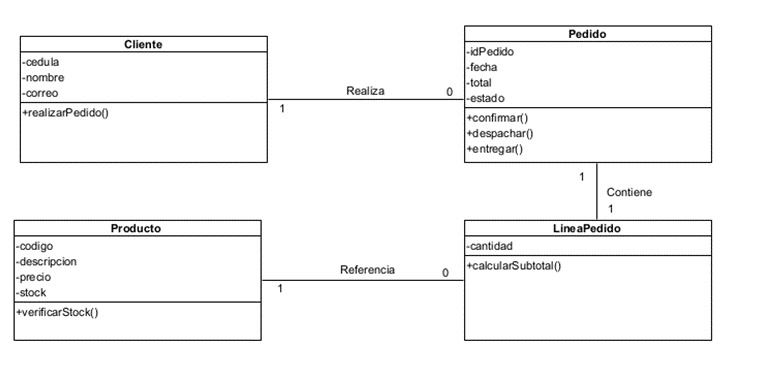
\includegraphics[width=0.85\textwidth]{diagrama_clases.jpeg}
\end{center}

% ----------------------- P4 -----------------------
\subsection*{P4. Consistencia entre las tres perspectivas}

Elabore una tabla de verificación cruzada que relacione cada evento de P3 con la función/acción
de P2 que lo realiza y con la entidad o atributo de P1 que modifica. Detecte al menos una
inconsistencia entre los modelos (evento sin función, entidad sin clase, etc.), documente el
defecto y corrija el modelo afectado.

\begin{center}
\begin{tabular}{|p{4cm}|p{4cm}|p{5cm}|}
\hline
\rowcolor{tablehead}
\textbf{Evento P3} & \textbf{Acción P2} & \textbf{Entidad/atributo de P1 modificado} \\
\hline
Registrar pedido & Registrar pedido & Pedido.estado = Registro \\
\hline
Confirmar pedido & Confirmar pedido & Pedido.estado = Confirmado \\
\hline
Despachar pedido & Despachar pedido & Pedido.estado = Despachado \\
\hline
Entregar pedido & Entregar pedido & Pedido.estado = Entregado \\
\hline
Anular pedido & Anular pedido & Pedido.estado = Anulado \\
\hline
Verificar Stock & Verificar disponibilidad & Producto.Stock \\
\hline
\end{tabular}
\end{center}

% ----------------------- P5 -----------------------
\subsection*{P5. Especificación de requisitos con esquema de atributos}

Redacte 4 requisitos: 2 funcionales y 2 no funcionales. Cada requisito no funcional debe nombrar
una característica de ISO/IEC 25010:2023 (p. ej. Eficiencia de desempeño, Seguridad), fijar una
métrica y un umbral (p. ej. ``registrar el pedido en $<$ 3 s''). Para cada requisito complete un
esquema de atributos: identificador, prioridad, estado, fuente, estabilidad, versión y método de
verificación.

\subsubsection*{Requisitos Funcionales}

\begin{requisito}{RF-01 --- Registrar pedido}
  \item[Identificador:] RF-01
  \item[Prioridad:] Alta
  \item[Estado:] Propuesto
  \item[Fuente:] Caso práctico
  \item[Estabilidad:] Funcional
  \item[Versión:] 1.0
  \item[Método de verificación:] Prueba funcional
\end{requisito}

\begin{requisito}{RF-02 --- Gestionar estado del pedido}
  \item[Identificador:] RF-02
  \item[Prioridad:] Alta
  \item[Estado:] Propuesto
  \item[Fuente:] Caso práctico
  \item[Estabilidad:] Funcional
  \item[Versión:] 1.0
  \item[Método de verificación:] Prueba funcional
\end{requisito}

\subsubsection*{Requisitos No Funcionales}

\begin{requisito}{RNF-01 --- Rendimiento}
  \item[Característica:] Eficiencia de desempeño
  \item[Identificador:] RNF-01
  \item[Prioridad:] Alta
  \item[Estado:] Propuesto
  \item[Fuente:] Caso práctico
  \item[Estabilidad:] No funcional
  \item[Versión:] 1.0
  \item[Método de verificación:] Prueba de rendimiento
\end{requisito}

\begin{requisito}{RNF-02 --- Seguridad}
  \item[Característica:] Seguridad
  \item[Identificador:] RNF-02
  \item[Prioridad:] Alta
  \item[Estado:] Propuesto
  \item[Fuente:] Caso práctico
  \item[Estabilidad:] No funcional
  \item[Versión:] 1.0
  \item[Método de verificación:] Inspección y prueba de seguridad
\end{requisito}

% ----------------------- P6 -----------------------
\subsection*{P6. Priorización MoSCoW}

Clasifique los 4 requisitos de P5 en las categorías MoSCoW (Must / Should / Could / Won't have
this time) y justifique brevemente cada asignación en función del valor y la viabilidad. Al menos
un requisito debe ser Must have.

\begin{center}
\begin{tabular}{|l|l|p{8cm}|}
\hline
\rowcolor{tablehead}
\textbf{Requisito} & \textbf{Prioridad} & \textbf{Justificación} \\
\hline
RF-01  & Must have   & Sin registrar el pedido, el sistema no cumple su función principal. \\
\hline
RF-02  & Must have   & Es necesario gestionar el ciclo de vida de los pedidos. \\
\hline
RNF-01 & Should have & El rendimiento rápido es importante para el sistema. \\
\hline
RNF-02 & Must have   & El sistema maneja datos personales y debe protegerlos. \\
\hline
\end{tabular}
\end{center}

% ----------------------- P7 -----------------------
\subsection*{P7. Validación por inspección (lista de comprobación 29148)}

Aplique a los requisitos de P5 una lista de comprobación derivada de las propiedades de
ISO/IEC/IEEE 29148 (no ambiguo, completo, singular, verificable, factible). Registre los defectos
detectados sin corregirlos en el momento (separar identificación de corrección) y, en un segundo
paso, presente el retrabajo con los requisitos corregidos.

\begin{center}
\begin{tabular}{|l|c|c|c|c|c|p{4cm}|}
\hline
\rowcolor{tablehead}
\textbf{ID} & \textbf{No ambiguo} & \textbf{Completo} & \textbf{Singular} & \textbf{Verificable} & \textbf{Factible} & \textbf{Defecto} \\
\hline
RF-01  & \cmark & \cmark & \cmark & \cmark & \cmark & Ninguno \\
\hline
RF-02  & \xmark & \cmark & \xmark & \cmark & \cmark & Mezcla varias acciones \\
\hline
RNF-01 & \cmark & \cmark & \cmark & \cmark & \cmark & Ninguno \\
\hline
RNF-02 & \xmark & \cmark & \cmark & \xmark & \cmark & No define claramente cómo verificar \\
\hline
\end{tabular}
\end{center}

\paragraph{Defectos encontrados}

Defecto RF-02: Contiene varias acciones: confirmar, despachar, entregar y anular.

Corrección: Dividirlo en requisitos independientes o definir el alcance para mantener solo
cuatro requisitos.

Defecto RNF-02: Inicialmente no tenía un criterio concreto de comprobación.

Corrección: Agregar un criterio concreto de comprobación.

% ----------------------- P8 -----------------------
\subsection*{P8. Pruebas de aceptación trazadas}

Defina una prueba de aceptación por requisito (4 en total), indicando su tipo (funcional, no
funcional o regresión), sus entradas, el criterio de éxito y el requisito al que traza. Cada
prueba debe enlazar explícitamente con al menos un requisito de P5.

\begin{center}
\begin{tabular}{|l|l|p{7cm}|}
\hline
\rowcolor{tablehead}
\textbf{ID} & \textbf{Tipo} & \textbf{Entrada} \\
\hline
PA-01 & Funcional    & Cliente, producto disponible y cantidad válida \\
\hline
PA-02 & Funcional    & Pedido registrado \\
\hline
PA-03 & No funcional & 100 usuarios registrando pedidos \\
\hline
PA-04 & No funcional & Usuarios autorizado / no autorizado \\
\hline
\end{tabular}
\end{center}

% ----------------------- P9 -----------------------
\subsection*{P9. Matriz de trazabilidad}

Construya la matriz de trazabilidad que cruce los requisitos con: su fuente (traza hacia atrás) y
sus modelos y pruebas de aceptación (traza hacia adelante). Marque también al menos una
dependencia horizontal entre requisitos e identifique cualquier requisito huérfano (sin prueba o
sin modelo asociado).

\begin{center}
\begin{tabular}{|l|l|p{7cm}|}
\hline
\rowcolor{tablehead}
\textbf{Requisitos} & \textbf{Fuente} & \textbf{Producto/Elemento} \\
\hline
RF-01  & Caso práctico & Cliente, Pedido, Línea de Pedido, Producto \\
\hline
RF-02  & Caso práctico & Pedido, Estado \\
\hline
RNF-01 & Caso práctico & Pedido \\
\hline
RNF-02 & Caso práctico & Cliente \\
\hline
\end{tabular}
\end{center}

\paragraph{Dependencia Horizontal}

RF-01 $\rightarrow$ RF-02

Primero debe existir un pedido para poder gestionarlo.

\paragraph{Requisitos huérfanos}

No existen requisitos huérfanos.

% ----------------------- P10 -----------------------
\subsection*{P10. Gestión del cambio y línea base}

Simule una solicitud de cambio sobre un requisito: regístrela, analice su impacto usando la
matriz de P9, indique la decisión del CCB (aprobada/rechazada/diferida) y actualice la versión
del requisito. Finalmente, declare una línea base: liste la configuración (versiones coherentes
de ERS, modelos, matriz y pruebas) que se congela.

\paragraph{SC-01:}
Se solicita modificar RNF-01 para mejorar el tiempo máximo de respuesta del registro de pedidos
de 3 segundos a 2 segundos.

\paragraph{Análisis de impacto}
\begin{itemize}[nosep]
  \item RNF-01
  \item P5 -- Especificación de requisitos
  \item P6 -- Priorización MoSCoW
  \item P7 -- Lista de comprobación
  \item P8 -- Prueba PA-03
  \item P9 -- Matriz de trazabilidad
\end{itemize}

\paragraph{Decisión del CCB}
Aprobada

Justificación: El cambio mejora el rendimiento de espera del sistema y es técnicamente viable.
Requiere actualizar la prueba de aceptación y verificar que la infraestructura pueda cumplir el
nuevo límite.

\paragraph{Nueva versión}
\begin{description}[leftmargin=0pt,style=sameline]
  \item[RNF-01 --- Versión anterior:] 1.0
  \item[Tiempo máximo (anterior):] $\leq$ 3 segundos
  \item[RNF-01 --- Nueva versión:] 1.1
  \item[Tiempo máximo (nuevo):] $\leq$ 2 segundos
\end{description}

\paragraph{Nueva prueba PA-03}
Con una carga de hasta 100 usuarios concurrentes, el sistema deberá registrar y confirmar en un
tiempo de respuesta menor o igual a 2 segundos.

\bigskip
\paragraph{Línea base}

\begin{center}
\begin{tabular}{|l|l|}
\hline
\rowcolor{tablehead}
\textbf{Elemento} & \textbf{Versión} \\
\hline
Requisito P5              & 1.1 \\
\hline
Diagrama de clases P1     & 1.0 \\
\hline
Diagrama de actividades P2 & 1.0 \\
\hline
Máquina de estados P3     & 1.0 \\
\hline
Matriz de trazabilidad    & 1.1 \\
\hline
Pruebas de aceptación P8  & 1.1 \\
\hline
\end{tabular}
\end{center}

\end{document}
